\documentclass[tikz,border=10pt]{standalone}
\usepackage{amsmath}
\begin{document}
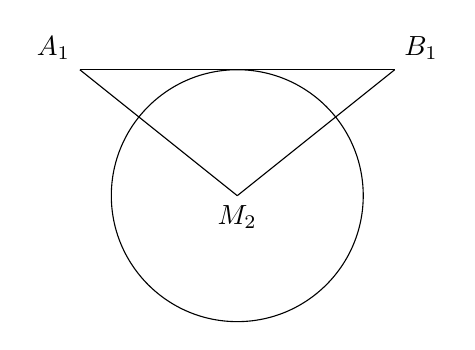
\begin{tikzpicture}[scale=0.04]
  % Points
  \coordinate (A1) at (0,100);
  \coordinate (B1) at (100,100);
  \coordinate (M2) at (50,60);

  % Circle centered at M2
  \coordinate (C) at (50,60);

  % Triangle edges (solid)
  \draw (A1) -- (B1);
  \draw (A1) -- (M2);
  \draw (B1) -- (M2);

  % Circle (solid)
  \draw (C) circle (40);

  % Labels
  \node[above left] at (A1) {$A_1$};
  \node[above right] at (B1) {$B_1$};
  \node[below] at (M2) {$M_2$};
\end{tikzpicture}
\end{document}
